\documentclass{article}
\usepackage{tikz}
\usepackage{CJKutf8}
\usepackage{amsmath}
\usepackage{amsthm}
\begin{document}
\begin{CJK}{UTF8}{gbsn}
\newtheorem{Exercise}{习题}
\begin{Exercise}
  画出具有$3$个顶点的所有有向图(同构的只算一个)。
\end{Exercise}
\centering
\begin{minipage}{0.24\linewidth}\centering
  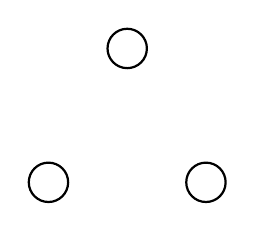
\begin{tikzpicture}[auto,
    specification/.style ={circle, draw, thick,inner sep=0pt, minimum size=5mm}]
   \node[specification] (A)  at (-1,0)  {};
   \node[specification] (B)  at (1,0)  {};
   \node[specification] (C)  at (0,1.7)  {};
 \end{tikzpicture}\\
  \vspace*{0.3cm}
  A
\end{minipage}\hfill
\begin{minipage}{0.24\linewidth}\centering
  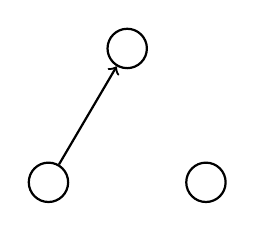
\begin{tikzpicture}[auto,
    specification/.style ={circle, draw, thick,inner sep=0pt, minimum size=5mm}]
   \node[specification] (A)  at (-1,0)  {};
   \node[specification] (B)  at (1,0)  {};
   \node[specification] (C)  at (0,1.7)  {};
   \draw[thick, ->] (A) to  (C);
 \end{tikzpicture}\\
   \vspace*{0.3cm}
B
\end{minipage}\hfill
 \begin{minipage}{0.24\linewidth}\centering
  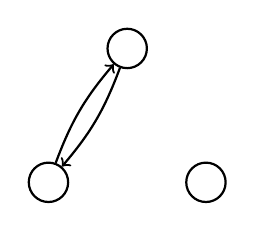
\begin{tikzpicture}[auto,
    specification/.style ={circle, draw, thick,inner sep=0pt, minimum size=5mm}]
   \node[specification] (A)  at (-1,0)  {};
   \node[specification] (B)  at (1,0)  {};
   \node[specification] (C)  at (0,1.7)  {};
   \draw[thick, ->] (A) to  [bend left=10] (C);
   \draw[thick, ->] (C) to  [bend left=10] (A);   
 \end{tikzpicture}\\
   \vspace*{0.3cm}
C
\end{minipage}\hfill
 \begin{minipage}{0.24\linewidth}\centering
  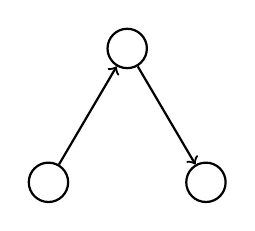
\begin{tikzpicture}[auto,
    specification/.style ={circle, draw, thick,inner sep=0pt, minimum size=5mm}]
   \node[specification] (A)  at (-1,0)  {};
   \node[specification] (B)  at (1,0)  {};
   \node[specification] (C)  at (0,1.7)  {};
   \draw[thick, ->] (A) to  (C);
   \draw[thick, ->] (C) to  (B);
 \end{tikzpicture}\\
   \vspace*{0.3cm}
D
\end{minipage}

\vspace{0.3cm}
 \begin{minipage}{0.24\linewidth}\centering
  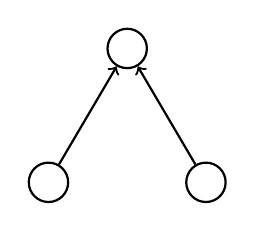
\begin{tikzpicture}[auto,
    specification/.style ={circle, draw, thick,inner sep=0pt, minimum size=5mm}]
   \node[specification] (A)  at (-1,0)  {};
   \node[specification] (B)  at (1,0)  {};
   \node[specification] (C)  at (0,1.7)  {};
   \draw[thick, ->] (A) to  (C);
   \draw[thick, ->] (B) to  (C);
\end{tikzpicture}\\
  \vspace*{0.3cm}
  E
\end{minipage}\hfill
 \begin{minipage}{0.24\linewidth}\centering
  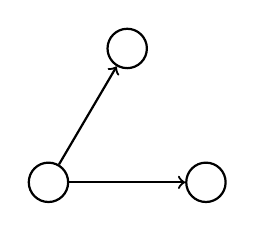
\begin{tikzpicture}[auto,
    specification/.style ={circle, draw, thick,inner sep=0pt, minimum size=5mm}]
   \node[specification] (A)  at (-1,0)  {};
   \node[specification] (B)  at (1,0)  {};
   \node[specification] (C)  at (0,1.7)  {};
   \draw[thick, ->] (A) to  (C);
   \draw[thick, ->] (A) to  (B);
\end{tikzpicture}\\
  \vspace*{0.3cm}
  F
\end{minipage}\hfill
 \begin{minipage}{0.24\linewidth}\centering
  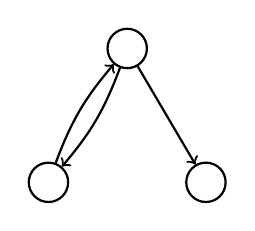
\begin{tikzpicture}[auto,
    specification/.style ={circle, draw, thick,inner sep=0pt, minimum size=5mm}]
   \node[specification] (A)  at (-1,0)  {};
   \node[specification] (B)  at (1,0)  {};
   \node[specification] (C)  at (0,1.7)  {};
   \draw[thick, ->] (A) to  [bend left=10] (C);
   \draw[thick, ->] (C) to  [bend left=10] (A);
   \draw[thick, ->] (C) to  (B);   
\end{tikzpicture}\\
  \vspace*{0.3cm}
  G
\end{minipage}\hfill
 \begin{minipage}{0.24\linewidth}\centering
  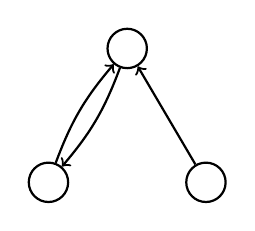
\begin{tikzpicture}[auto,
    specification/.style ={circle, draw, thick,inner sep=0pt, minimum size=5mm}]
   \node[specification] (A)  at (-1,0)  {};
   \node[specification] (B)  at (1,0)  {};
   \node[specification] (C)  at (0,1.7)  {};
   \draw[thick, ->] (A) to  [bend left=10] (C);
   \draw[thick, ->] (C) to  [bend left=10] (A);
   \draw[thick, ->] (B) to  (C);
 \end{tikzpicture}\\
  \vspace*{0.3cm}
  H
\end{minipage}

\vspace{0.3cm}
 \begin{minipage}{0.24\linewidth}\centering
  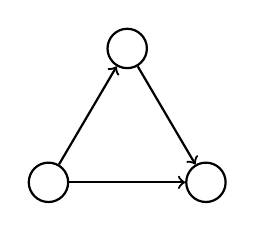
\begin{tikzpicture}[auto,
    specification/.style ={circle, draw, thick,inner sep=0pt, minimum size=5mm}]
   \node[specification] (A)  at (-1,0)  {};
   \node[specification] (B)  at (1,0)  {};
   \node[specification] (C)  at (0,1.7)  {};
   \draw[thick, ->] (A) to  (C);
   \draw[thick, ->] (C) to  (B);
   \draw[thick, ->] (A) to  (B);   
\end{tikzpicture}\\
  \vspace*{0.3cm}
  I
\end{minipage}\hfill
 \begin{minipage}{0.24\linewidth}\centering
  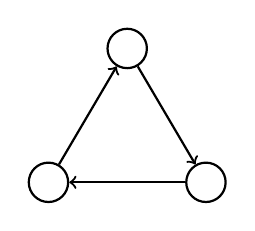
\begin{tikzpicture}[auto,
    specification/.style ={circle, draw, thick,inner sep=0pt, minimum size=5mm}]
   \node[specification] (A)  at (-1,0)  {};
   \node[specification] (B)  at (1,0)  {};
   \node[specification] (C)  at (0,1.7)  {};
   \draw[thick, ->] (A) to  (C);
   \draw[thick, ->] (C) to  (B);
   \draw[thick, ->] (B) to  (A);
 \end{tikzpicture}\\
  \vspace*{0.3cm}
  J
\end{minipage}\hfill
 \begin{minipage}{0.24\linewidth}\centering
  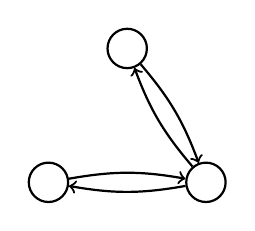
\begin{tikzpicture}[auto,
    specification/.style ={circle, draw, thick,inner sep=0pt, minimum size=5mm}]
   \node[specification] (A)  at (-1,0)  {};
   \node[specification] (B)  at (1,0)  {};
   \node[specification] (C)  at (0,1.7)  {};
   \draw[thick, ->] (A) to  [bend left=10] (B);
   \draw[thick, ->] (B) to  [bend left=10] (A);
   \draw[thick, ->] (B) to  [bend left=10] (C);
   \draw[thick, ->] (C) to  [bend left=10] (B);
 \end{tikzpicture}\\
  \vspace*{0.3cm}
  K
\end{minipage}\hfill
 \begin{minipage}{0.24\linewidth}\centering
  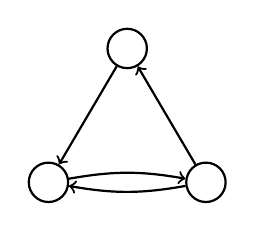
\begin{tikzpicture}[auto,
    specification/.style ={circle, draw, thick,inner sep=0pt, minimum size=5mm}]
   \node[specification] (A)  at (-1,0)  {};
   \node[specification] (B)  at (1,0)  {};
   \node[specification] (C)  at (0,1.7)  {};
   \draw[thick, ->] (A) to  [bend left=10] (B);
   \draw[thick, ->] (B) to  [bend left=10] (A);
   \draw[thick, ->] (B) to  (C);
   \draw[thick, ->] (C) to  (A);
 \end{tikzpicture}\\
  \vspace*{0.3cm}
  L
\end{minipage}

\vspace{0.3cm}
 \begin{minipage}{0.24\linewidth}\centering
   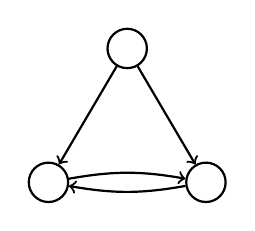
\begin{tikzpicture}[auto,
    specification/.style ={circle, draw, thick,inner sep=0pt, minimum size=5mm}]
   \node[specification] (A)  at (-1,0)  {};
   \node[specification] (B)  at (1,0)  {};
   \node[specification] (C)  at (0,1.7)  {};
   \draw[thick, ->] (A) to  [bend left=10] (B);
   \draw[thick, ->] (B) to  [bend left=10] (A);
   \draw[thick, ->] (C) to  (B);
   \draw[thick, ->] (C) to  (A);
 \end{tikzpicture}\\
  \vspace*{0.3cm}
  M
\end{minipage}\hfill
 \begin{minipage}{0.24\linewidth}\centering
  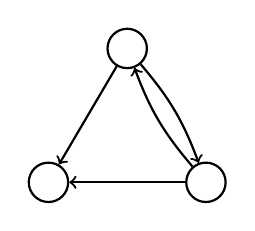
\begin{tikzpicture}[auto,
    specification/.style ={circle, draw, thick,inner sep=0pt, minimum size=5mm}]
   \node[specification] (A)  at (-1,0)  {};
   \node[specification] (B)  at (1,0)  {};
   \node[specification] (C)  at (0,1.7)  {};
   \draw[thick, ->] (C) to   (A);
   \draw[thick, ->] (B) to   (A);
   \draw[thick, ->] (B) to  [bend left=10] (C);
   \draw[thick, ->] (C) to  [bend left=10] (B);
 \end{tikzpicture}\\
  \vspace*{0.3cm}
  N
\end{minipage}\hfill
 \begin{minipage}{0.24\linewidth}\centering
  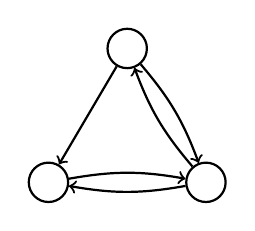
\begin{tikzpicture}[auto,
    specification/.style ={circle, draw, thick,inner sep=0pt, minimum size=5mm}]
   \node[specification] (A)  at (-1,0)  {};
   \node[specification] (B)  at (1,0)  {};
   \node[specification] (C)  at (0,1.7)  {};
   \draw[thick, ->] (A) to  [bend left=10] (B);
   \draw[thick, ->] (B) to  [bend left=10] (A);
   \draw[thick, ->] (B) to  [bend left=10] (C);
   \draw[thick, ->] (C) to  [bend left=10] (B);
   \draw[thick, ->] (C) to   (A);   
 \end{tikzpicture}\\
  \vspace*{0.3cm}
  O
\end{minipage}\hfill
 \begin{minipage}{0.24\linewidth}\centering
  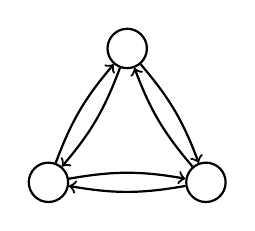
\begin{tikzpicture}[auto,
    specification/.style ={circle, draw, thick,inner sep=0pt, minimum size=5mm}]
   \node[specification] (A)  at (-1,0)  {};
   \node[specification] (B)  at (1,0)  {};
   \node[specification] (C)  at (0,1.7)  {};
   \draw[thick, ->] (A) to  [bend left=10] (B);
   \draw[thick, ->] (B) to  [bend left=10] (A);
   \draw[thick, ->] (B) to  [bend left=10] (C);
   \draw[thick, ->] (C) to  [bend left=10] (B);
   \draw[thick, ->] (A) to  [bend left=10] (C);
   \draw[thick, ->] (C) to  [bend left=10] (A);   
 \end{tikzpicture}\\
  \vspace*{0.3cm}
  P
\end{minipage}

\begin{Exercise}
  具有$p$个顶点的完全有向图中有多少条弧?
\end{Exercise}
\begin{proof}[解]
  $p(p-1)$。
\end{proof}
\begin{Exercise}
  设$D$为一个有$p$个顶点$q$条弧的有向图。如果$D$为连通的,证明:$p-1\leq q \leq p(p-1)$。
\end{Exercise}
\begin{Exercise}
  设$D$为一个有$p$个顶点$q$条弧的强连通的有向图,则$q$至少是多大?
\end{Exercise}
\begin{proof}[答]
  当$p=1$时,$q=0$;当$p>1$时,$q$至少为$p$。

  当$p>1$时,设$u$和$v$为$D$的两个顶点,由$D$为强连通的知从$u$到$v$有一条有向路$uu_1u_2\ldots u_nv$,从$v$到$u$有一条有向路$vu_{n+2}u_{n+3}\ldots u_{n+m}u$。
  考虑有向闭通道$W=uu_1u_2\ldots u_nvu_{n+2}u_{n+3}\ldots u_{n+m}u$,记$u_0=u$,$v_{n+1}=v$。设$u_j$为$W$上第一个与前面的某个顶点$u_i$重复的顶点,那么$u_iu_{i+1}\ldots u_j$构成了$D$中的一个圈。这证明了当$p>1$时,任意一个强连通图中必定有圈。因此,抹去$D$中所有弧的方向所得到的无向图为连通的,且至少有$1$个圈,去掉该圈上的一条边,所得到的无向图仍然为连通的,从而$q-1\geq p-1$,即$q\geq p$。

  显然由$p$个顶点$v_1,v_2,\ldots,v_p$依次相连所构成的圈$v_1v_2\ldots v_pv_1$有$p$条弧。因此$q$至少为$p$。
 
\end{proof}

\begin{Exercise}
  有向图$D$的图解如下图所示:
  
  \centering
  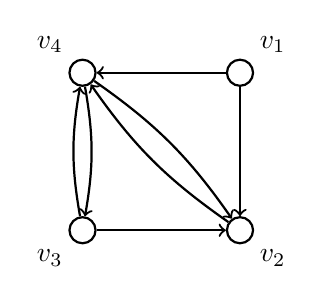
\begin{tikzpicture}[auto,
    specification/.style ={circle, draw, thick}]
   \node[specification] (A) [label=-135:$v_3$] at (0,0)  {};
   \node[specification] (B) [label=135:$v_4$] at (0,2)  {};
   \node[specification] (C) [label=45:$v_1$] at (2,2)  {};
   \node[specification] (D) [label=-45:$v_2$] at (2,0)  {};
   \draw[thick, ->] (A) to  (D);
   \draw[thick, ->] (C) to  (B);
   \draw[thick, ->] (C) to  (D);
   \draw[thick, ->] (A) to [bend left = 10] (B);
   \draw[thick, ->] (B) to [bend left = 10] (A);
   \draw[thick, ->] (B) to [bend left = 10] (D);
   \draw[thick, ->] (D) to [bend left = 10] (B);   
 \end{tikzpicture}\hspace{1cm}\\
 D

 \begin{enumerate}
  \renewcommand{\labelenumi}{(\theenumi)}
  \item 写出$D$的邻接矩阵及可达矩阵;
  \item 写出$D$的关联矩阵。
  \end{enumerate}
\end{Exercise}
\begin{proof}[解]
  D的邻接矩阵:\[\begin{bmatrix}0&1&0&1\\0&0&0&1\\0&1&0&1\\0&1&1&0\end{bmatrix}\]
  D的可达矩阵:\[\begin{bmatrix}1&1&1&1\\0&1&1&1\\0&1&1&1\\0&1&1&1\end{bmatrix}\]
  D的关联矩阵:\[\begin{bmatrix}1&1&0&0&0&0&0\\-1&0&0&-1&-1&0&1\\0&0&1&1&0&-1&0\\0&-1&-1&0&1&1&-1\end{bmatrix}\]
\end{proof}

\begin{Exercise}
  有向图$D$的图解如下图所示:

  \centering
  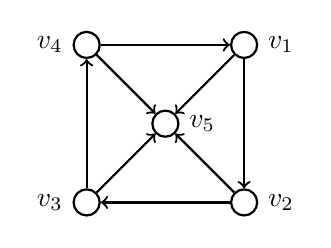
\begin{tikzpicture}[auto,
    specification/.style ={circle, draw, thick}]
   \node[specification] (A) [label=0:$v_1$] at (1,1)  {};
   \node[specification] (B) [label=0:$v_2$] at (1,-1)  {};
   \node[specification] (C) [label=180:$v_3$] at (-1,-1)  {};
   \node[specification] (D) [label=180:$v_4$] at (-1,1)  {};
   \node[specification] (E) [label=0:$v_5$] at (0,0)  {};
   
   \draw[thick, ->] (A) to  (B);
   \draw[thick, ->] (B) to  (C);
   \draw[thick, ->] (C) to  (D);
   \draw[thick, ->] (D) to  (A);
   \draw[thick, ->] (A) to  (E);
   \draw[thick, ->] (B) to  (E);
   \draw[thick, ->] (C) to  (E);
   \draw[thick, ->] (D) to  (E);   
 \end{tikzpicture}\hspace{1cm}\\
 D

求从顶点$v_2$到其余每个顶点的长$\leq 4$的所有有向通道的条数。 
\end{Exercise}
\begin{Exercise}
  设$T$为一棵正则$m$元有序树,它有$n_0$个叶子,$T$有多少条弧?
\end{Exercise}
\begin{proof}[解]
  当$m=1$时,$T$可以有任意正整数条弧;当$m>1$时,$T$有$\frac{m(n_0-1)}{m-1}$条弧。
\end{proof}
\begin{Exercise}
  设$T$为一棵有$n_0$个叶子的二元树,出度为$2$的顶点数为$n_2$,试证$n_0=n_2+1$。
\end{Exercise}
\begin{proof}[证明]
  设出度为$1$的顶点数为$n_1$,则$2n_2+n_1=n_2+n_1+n_0-1$,从而$n_0=n_2+1$。
\end{proof}
\begin{Exercise}
  用数学归纳法证明每个比赛图中必有有向哈密顿路。
\end{Exercise}
\begin{proof}[证明]
  用数学归纳法证明,施归纳于顶点数$p$。

  (1)当$p=1$时,结论显然成立。

  (2)假设当$p=k(k\geq 1)$时结论成立,往证当$p=k+1$时结论也成立。设$D=(V,A)$为一个包含$k+1$个顶点的比赛图,$v$为$D$的任意一个顶点,则$D-v$为一个包含$k$个顶点的比赛图。由归纳假设,$D-v$有一条有向哈密顿路$v_1v_2\ldots v_k$。如果$(v,v_1)\in A$,那么$vv_1v_2\ldots v_k$为有向图$D$的一条有向哈密顿路;如果$(v_k,v)\in A$,那么$v_1v_2\ldots v_kv$为有向图$D$的一条有向哈密顿路;如果$(v,v_1)\notin A$并且$(v_k,v)\notin A$,由$D$为比赛图知$(v_1,v)\in A$并且$(v,v_k)\in A$,在$1,2,\ldots, k$中选取最大的下标$i$使得$(v_i,v)\in A$,则$(v,v_{i+1})\in A$,于是$v_1, v_2,\ldots,v_i,$ $v,v_{i+1},\ldots,v_k$为$D$的一条有向哈密顿路。 
\end{proof}

\end{CJK}
\end{document}


%%% Local Variables:
%%% mode: latex
%%% TeX-master: t
%%% End:
